\documentclass[12pt]{ociamthesis}  % default square logo 
\usepackage[spanish]{babel} 
\usepackage[utf8]{inputenc}
%\documentclass[12pt,beltcrest]{ociamthesis} % use old belt crest logo
%\documentclass[12pt,shieldcrest]{ociamthesis} % use older shield crest logo

%load any additional packages
\usepackage{amssymb}

%input macros (i.e. write your own macros file called mymacros.tex 
%and uncomment the next line)
%\include{mymacros}
\begin{document}

%this baselineskip gives sufficient line spacing for an examiner to easily
%markup the thesis with comments
\baselineskip=18pt plus1pt


%set the number of sectioning levels that get number and appear in the contents
\setcounter{secnumdepth}{3}
\setcounter{tocdepth}{2}


%\maketitle                  % create a title page from the preamble info
\begin{titlepage}
	\begin{center}
		
\includegraphics[width=5cm]{logo2.png}\\
		\vspace{1cm}
		FACULTAD DE INGENIERÍA\\
		INGENIERÍA CIVIL INFORMÁTICA\\
		\vspace{1cm}
		\LARGE{\textbf{Una arquitectura caché para redes ICN basada en comportamiento de usuario} \\}
		\vspace{1cm}
		\small{Tesis para optar al grado de ingeniero civil en informática.}\\
		\vspace{2cm}
		\textbf{Autor:} \\
		Mathias Nicolas Velilla Brandau.\\
		\vspace{1cm}
		\textbf{Profesores guía:} \\
		Carlos Gomez-Pantoja\\
		Miguel Guitierrez\\
		\vspace{1cm}
		Santiago de Chile, Chile.\\
		\vspace{1cm}
		Abril, 2017
	\end{center}
\end{titlepage}


\begin{romanpages}          % start roman page numbering
\tableofcontents            % generate and include a table of contents
\listoffigures              % generate and include a list of figures
\end{romanpages}            % end roman page numbering

\chapter{Introducción}
\section{Motivación}

El nacimiento del Internet en el año 1958 en EE.UU. a través de ARPA (\textit{Advanced Researchs Proyects Agency}) tuvo como objetivo la comunicación entre diversas entidades con propósitos investigativos, la aparición de la conmutación por paquetes implementadas en los mecanismos de comunicación sentó las bases para el desarrollo de esta nueva tecnología, la cual hoy en día ha revolucionado la informática y las comunicaciones como ninguna otra cosa, convirtiéndose en una herramienta de índole mundial, un mecanismo el cual nos permite diseminar información de manera inmediata , generando un medio de colaboración e interacción entre las personas y los ordenadores, desconociendo su ubicación física.\\

Durante los año 2000 - 2008 el uso diario del Internet en las personas americanas redondeaba entre un 60\% y 70\% [Digital Citize], este aumento en el uso de la Internet, conlleva también a un aumento de la información presente en la web, dando como resultado el desarrollo de aplicaciones las cuales deben interactuar con un gran numero de usuarios y analizando una sobresaliente cantidad de información, motivo por el cual Internet impulsado por las demandas de las aplicaciones cada vez más emergentes y las capacidades de las nuevas redes de comunicación, se ha convertido en un mosaico arquitectónico que resulta en una creciente complejidad y vulnerabilidades imprescindibles, entregando como resultado violaciones de capas, proliferación de subcapas, y la erosión del modelo de extremo a extremo, es bajo esta eventualidad que todos los cambios efectuados concluyen en un aumento de la complejidad, lo cual se traduce en una Internet osificada, es por esta razón que los problemas anteriormente señalados no se encuentran directamente relacionados con los protocolos o mecanismo específicos del Internet actual, mas bien son causados esencialmente por la incapacidad de integrar nuevos mecanismos, lo que quiere decir que los problemas son causados por la arquitectura de Internet y podrían ser resueltos con un nuevo diseño de arquitectura de Internet \cite{muller2009future}.\\

La creciente demanda de una distribución altamente escalable y eficiente del contenido ha motivado el desarrollo de futuras arquitecturas de Internet basadas en objetos de datos nombrados (NDO, por sus siglas en inglés), por ejemplo, páginas web, videos, documentos u otras informaciones. El enfoque de estas arquitecturas se conoce comúnmente como redes centradas en información (ICN). Por el contrario, las redes actuales se centran en el host, donde la comunicación se basa en hosts nombrados, por ejemplo, servidores web, PC, portátiles, teléfonos móviles y otros dispositivos\cite{ahlgren2012survey}.\\

Las arquitecturas ICN aprovechan el almacenamiento en red para el almacenamiento en caché, la comunicación multilateral a través de la replicación y los modelos de interacción que desacoplan a los remitentes y receptores. El objetivo común es lograr una distribución eficiente y confiable de los contenidos en donde cada uno de estos es nombrado única e independientemente desde la ubicación del productor(servidor), facilitando el almacenamiento en cache en los nodos intermediarios. Así, por ejemplo, los consumidores solicitaran contenidos enviando el denominado paquete de interés, el cual lleva el nombre del contenido, mientras que el productor o cualquier nodo que mantenga una copia del contenido puede responder a la petición realizada.\cite{ahlgren2012survey}\\

A su vez, los usuarios ya antes mencionados como consumidores, realizan peticiones en la web, las cuales siguen una conducta dinámica caracterizándose por un elevado sesgo entre los diferentes conjuntos de peticiones, en otras palabras, dentro del universo de peticiones generadas existen conjuntos de peticiones que son regularmente solicitadas por los consumidores en intervalos de tiempos distintos, por lo contrario, otras peticiones escasamente son solicitadas. Dicho lo anterior, también existen situaciones dentro de un intervalo acotado de tiempo, donde surgen explosiva mente peticiones las que se caracterizan por poseer un contenido en común, las cuales nacen por el desarrollo de un evento de interés popular teniendo como resultado un aumento sustancial en la demanda generada a los nodos, teniendo como consecuencia latencia y congestión en las redes.


\section{Desafíos}
%*******************************************************
Los desafíos que se afrontaran para la realización de proyecto de titulo I, son inicialmente el diseño de una nueva arquitectura de memoria caché para los nodos de las redes \textit{ICN} (\textit{Information Centric Network}), considerando el comportamiento de los usuarios por medio del tráfico de red. En segundo lugar, se debe incorporar una estrategia de caché(políticas de admisión, desalojo y reemplazo) y que será implementada en un simulador denominado \textit{ndnSIM} (\textit{Named Data Networking Simulator}), todo esto con el fin de mejorar resultados(Queresultados) en comparación con otras arquitecturas caché que se encuentran por defecto dentro del simulador(LFU, FIFO).\\

\section{Contribución de la tesis}
El aporte entregado por el proyecto de titulo, se puede identificar inicialmente por la creación diseño de una nueva arquitectura de memoria caché para los nodos de las redes \textit{ICN} (\textit{Information Centric Network}), considerando el comportamiento de los usuarios por medio del tráfico de red. En segundo lugar, se debe incorporar una estrategia de caché(políticas de admisión, desalojo y reemplazo) y que será implementada en un simulador denominado \textit{ndnSIM} (\textit{Named Data Networking Simulator}), todo esto con el fin de mejorar resultados de eficiencia de la memoria caché (Hit's, Miss) en comparación con otras arquitecturas caché que se encuentran por defecto dentro del simulador(LFU, FIFO). No obstante, a continuación se detallaran las contribuciones efectuadas por este trabajo:\\
\begin{itemize}
	\item Diseño de una nueva arquitectura cache bajo el paradigma de las redes ICN, que contenga una subdivisión de tres grupos capaces de retener diferentes tipos de peticiones(intereses) de modo que la eficiencia del nodo se vea afectada positivamente. En cuanto a la división de la memoria caché, el primer segmento se encarga del almacenamiento de peticiones del tipo ráfaga, la segunda de guardar las de tipo permanente y para la ultima sección, la recaudación de peticiones de tipo variables.\\
	\item Creación de una topologia de redes ICN, utilizando el simulador ndnSIM, la cual contenga dentro de sus nodos la arquitectura caché anteriormente señalada con la finalidad de inyectar trafico de datos en base al comportamiento usuario para la obtención de resultados empíricos respecto a la nueva arquitectura caché diseñada.\\
\end{itemize}


\section{Estructura de la tesis}
A continuación se realizara una breve reseña de como se estructura el siguiente trabajo:\\

El capitulo 2 abarca la descripción del problema, en el se define el objetivo general, específicos, hipótesis y los alcances que contiene el proyecto de titulo. Incluyendo también la descripción de la metodología de trabajo utilizada para el progreso del trabajo.\\

El capitulo 3 posee el marco teórico, en el cual se definen diferentes conceptos esenciales para el entendimiento del proyecto del titulo. Dicho lo anterior se encuentran los siguiente conceptos: Redes centradas en la información (ICN), ndnSIM, aplicaciones web de gran escala,el cache, estructura y políticas de remplazo del caché existentes y finalizando con el comportamiento del usuario de manera donde se explica la ley de Zipf y se detallan los tipos de peticiones de usuario.\\

En el capítulo 4 se presenta una revisión bibliográfica de los trabajos realizados respecto a las arquitecturas cache y las políticas de cache implementadas en redes ICN, ademas del revisión de trabajos dentro del simulador ndnSIM, todo esto con el fin de diseñar una arquitectura de cache que no exista en la literatura.\\

\chapter{Descripción del problema}

\section{Contextualización}
-¿Que es el cache y para que sirve?
\section{El problema}
\subsection{Declaración del problema}
\subsection{Diagrama de ishikawa}

\section{Objetivos}
\subsection{Objetivo general}
Optimizar la eficiencia del cache en redes \textit{ICN}, por medio del diseño de una arquitectura caché basada en el comportamiento de los usuarios, dentro del simulador \textit{ndnSIM}.

\subsection{Objetivos específicos}
\begin{itemize}
	\item Determinar los componentes estructurales de las redes \textit{ICN}.
	\item Proponer una arquitectura caché para redes \textit{ICN} que considere el comportamiento usuario.
	\item Incorporar una arquitectura cache en el simulador \textit{ndnSIM}
	\item Comparar el rendimiento de la estrategia caché propuesta con estrategias de la literatura
\end{itemize}

\subsection{Alcance de los objetivos}

\chapter{Marco teórico}

\section{Information Centric Network}
ICN (Information-Centric Networking) es un paradigma que pretende motivar la transición arquitectónica de la actual arquitectura centrada en el host a centrada en la información para difundir de manera eficiente y flexible la enorme información generada por una variedad de aplicaciones. En esta dirección de investigación, se han propuesto muchos enfoques durante los últimos años, de los cuales para el desarrollo de este trabajo nos centraremos en NDN.(Figura 3.1)
	\begin{figure}[!htb]
		\centering
		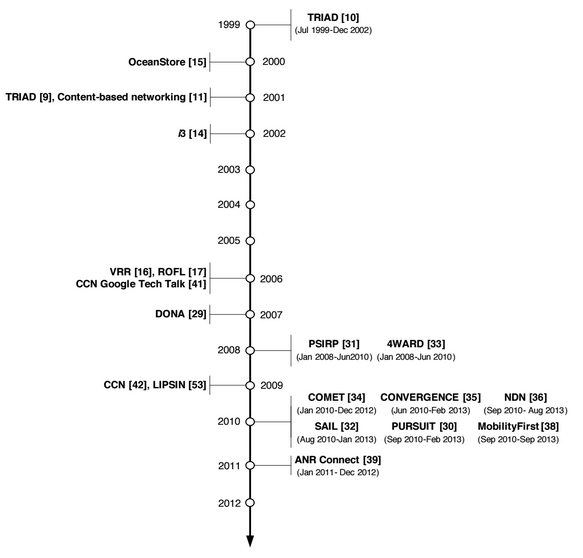
\includegraphics[width=10.2cm]{Linea_Temporal_ICN.png}\\
		\caption{Cronología de los principales hitos de ICN \cite{xylomenos2014survey}.}
		\label{fig:mesh1}
	\end{figure}

Named Data Networking (NDN) es una de las arquitecturas futuras para el internet con años de investigación sobre el uso de la red y de los problemas no resueltos en arquitecturas contemporáneas del internet como IP\cite{nsf10528}\cite{nsf13538}. La arquitectura NDN tiene su origen en el proyecto Content-Centric Networking (CCN) que Van Jacobson divulgo por primera vez en el año 2006 en una charla tecnológica de Google \cite{jacobson2006new}.\\

El proyecto NDN financiado por EE.UU desarrolla aun más la arquitectura CCN anteriormente mencionada, reconfigurando la pila de protocolos del internet haciendo el intercambio en la cintura delgada de la arquitectura de internet por el de datos nombrados y empleando diversas tecnologías de red por debajo de la cintura para la conectividad, incluyendo IP. También, NDN con el fin de optimizar el uso de recursos, contiene una capa de estrategia media que se ubica entre la capa de datos nombrada y las tecnologías de red, mientras que una capa de seguridad lleva a cabo las funcionalidad de seguridad directamente a los datos nombrados \cite{xylomenos2014survey} .(Figura 3.2)\\

	\begin{figure}[!htb]
		\centering
		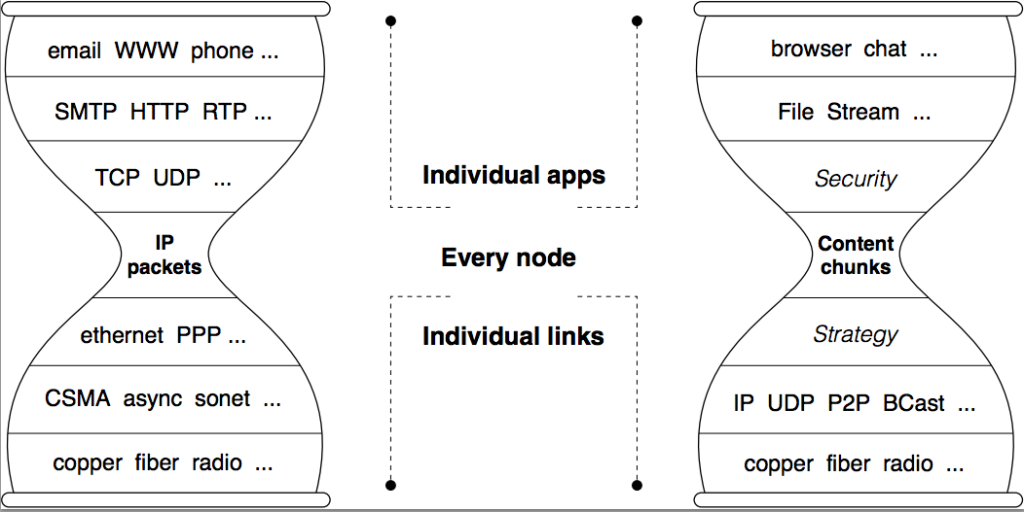
\includegraphics[width=12cm]{Protocolo_IP_vs_NDN.png}\\
		\caption{Arquitecturas de reloj de arena de Internet y NDN \cite{named_data_networking}.}
		\label{fig:mesh1}
	\end{figure}

Dicho lo anterior, la principal abstracción de ICN es el NDO (Named Data Objects), la que se define como la unidad de datos direccionales que se encuentra dentro de una red centrada en la información, siendo capaces de representar una colección de bytes o una información en especifica. Así mismo cada uno de los objetos de datos existentes posee un nombre vinculado a el, pudiendo verse como fragmentos de datos nombrados sin semántica alguna caracterizándose por su granularidad la cual varia desde el tamaño del paquete hasta los objetos completos \cite{kutscher2016information}\cite{ahlgren2012survey}.\\

Los objetos de datos con nombre se desligan de la ubicación, la aplicación, el almacenamiento y los medios de los transporte, dando paso al almacenamiento en cache y un bajo costo y ubicua replicación en la red, esperando como resultado una mayor eficiencia y seguridad, una mayor escabilidad respecto a la demanda de información/ancho de banda y una superior robustez en escenarios de comunicación desafiantes \cite{kutscher2016information}.\\

La arquitectura NDN se compone de dos tipos de NDO, los paquetes de interés(Interest Packet) y los paquetes de datos(Data Packet)(Figura 3.3), siendo el nombre de estos de tipo jerárquico, similares a una URL, como por ejemplo /aueb.gr/ai/main.html.

los cuales son enviados por dos tipos de usuarios el primero denominado consumidor,entidad encargada de enviar una solicitud de un NDO a la red(Interest) y por otra parte un productor, que es la entidad encargada publicar NDO's en la red, los cuales serán solicitados por un consumidor y enviados (Data).\\

\begin{figure}[!htb]
		\centering
		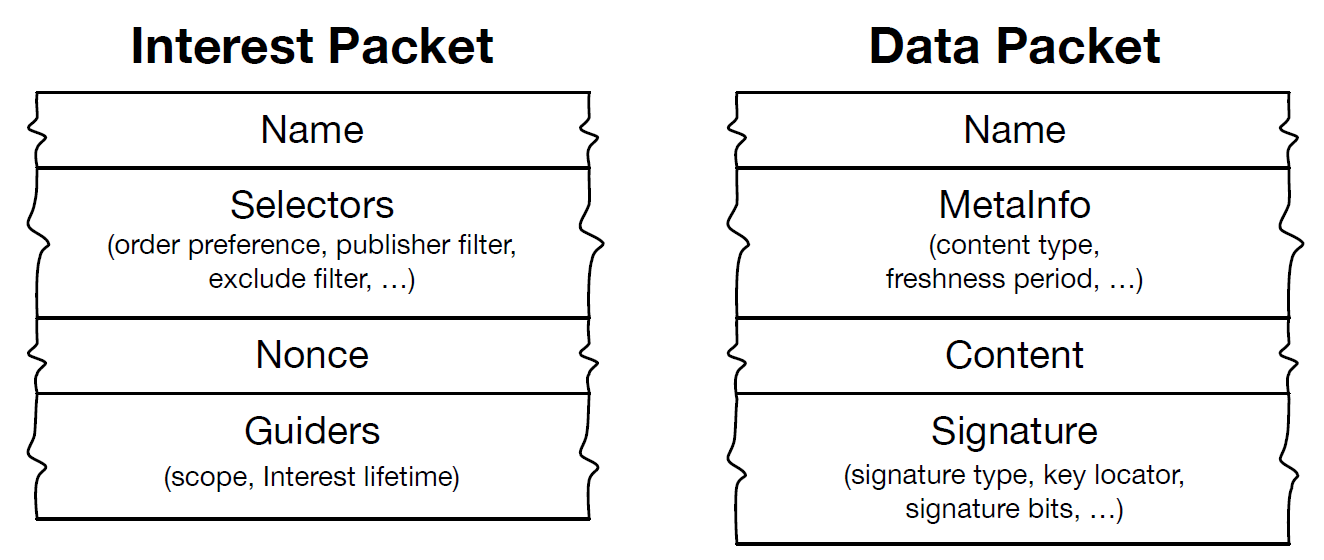
\includegraphics[width=10cm]{Paquetes_NDN.png}\\
		\caption{Paquetes NDN}
		\label{fig:mesh1}
\end{figure}
 
Adicionalmente esta arquitectura también cuenta con nodos intermediarios entre los consumidores y los productores denominados CR (Content Routers), lo cuales le entregan a la red un aumento en la replicación de información y consigo una mayor resolución de consultas. Los nodos contienen tres estructuras de datos principales(Figura 3.4):

\begin{itemize}
	\item\textbf{Forwarding Information Base (FIB):} El FIB se utiliza para reenviar paquetes de interés hacia fuentes potenciales de datos coincidentes. Es casi idéntico a un IP FIB, excepto que permite una lista de caras salientes en lugar de una sola. Esto refleja el hecho de que CCN no está restringido a reenvío en un árbol de expansión. Permite múltiples fuentes de datos y puede consultarlas todas en paralelo \cite{jacobson2009networking}.\\
	\item \textbf{Almacen de contenido (Content Store (CS):} El almacenamiento en caché de los NDO es una parte integral del servicio ICN. Todos los nodos potencialmente tienen cachés, incluyendo nodos en redes de infraestructura de ejecución de operadores y redes domésticas dirigidas por usuarios, así como terminales móviles. Las solicitudes de NDO pueden ser satisfechas por cualquier nodo que contenga una copia en su caché. ICN combina así el almacenamiento en caché en el borde de la red, como en P2P y otras redes de superposición, con almacenamiento en caché en la red (por ejemplo, cachés de web transparentes). El almacenamiento en caché es genérico, es decir, es independiente de la aplicación y se aplica a todos los proveedores de contenido, incluido el contenido generado por el usuario \cite{jacobson2009networking}.\\
	\item \textbf{Pending Interest Table (PIT):} El PIT realiza un seguimiento de los Intereses enviados hacia arriba hacia la(s) fuente(es) de contenido de forma que los datos devueltos puedan ser enviados aguas abajo a su(s) solicitante(s) \cite{jacobson2009networking}.\\
\end{itemize}

	\begin{figure}[!htb]
		\centering
		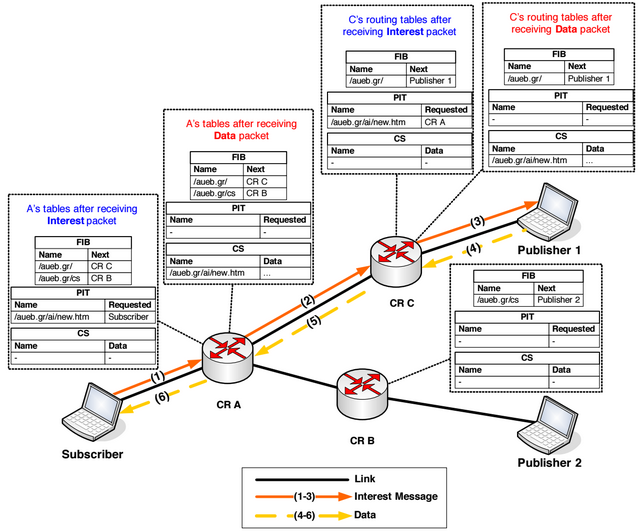
\includegraphics[width=10cm]{Nodo2.png}\\
		\caption{Nodo CCN}
		\label{fig:mesh1}
	\end{figure}


\section{Caché}
La cantidad de usuarios van en aumento día a día, por lo que las aplicaciones web con un gran numero de usuarios tienen que ser capaces de soportar grandes volúmenes de consultas y transacciones de datos(millones), las cuales poseen una patrón de comportamiento definido, este tema se abordara en (). Una de las tecnologías que existe para apaciguar el acceso incesante a información de los servidores, es la de un lugar de almacenamiento destinado a archivar las consultas y su respuesta pre-computada, denominado \textit{caché}.

El \textit{caché} es una de las partes mas importante dentro de los servicios web y motores de búsqueda \cite{altingovde2009cost},\cite{aggarwal1999caching}. Principalmente el cache es un espacio de almacenamiento(memoria) de acceso rápido, en donde se retienen las consultas más reiteradas hechas por los usuarios y sus respuestas, entregando una gran cantidad de ventajas entre las que se encuentran:

\begin{itemize}
	
	\item Reducir la latencia de acceso a los documentos, esto se debe a que los objetos que son accedidos con mayor frecuencia se encuentran almacenados en un nodo de cache cercano, lo que disminuye el tráfico en la red, permitiendo que los objetos que no están en cache puedan también ser recuperados con mayor rapidez \cite{wang1999survey}.
	
	\item Reducir el consumo de ancho de banda, lo que permite disminuir la congestión y el tráfico en la red \cite{wang1999survey}.
	
	\item Reducir la carga de trabajo en los servidores web \cite{wang1999survey}.
	
\end{itemize}

Siendo las características codiciables para una arquitectura cache las siguientes: robustez(capaz de no generar fallos o bloquearse), acceso rápido (disminuir latencia), eficiente, escalable, estable, adaptable y simple de implementar \cite{wang1999survey}. Por ello una de las finalidades más importante en el \textit{caché} es la de obtener el mayor numero respecto a la tasa de hit, en otras palabra, conseguir que una gran parte de las consultas realizadas por el usuario, que ingresan al cache cuente con una respuesta pre-computada.\\

En la arquitectura NDN, el caché de los CR juega un rol importante al momento de satisfacer las peticiones del usuario(Consumidor). A modo de que sin la presencia del cache, el paradigma de las redes ICN no seria valida, causando así que los productores(Servidores), procesen un volumen elevado de consultas simultaneas.La importancia del caché en la arquitectura NDN de las redes ICN radica en que esta requiere de una difuminación eficiente de la gran cantidad de consultas realizadas diariamente por lo usuarios, de manera que sean respondidas de forma rapida.\\

El cache es limitado, por lo que al completar su capacidad máxima es necesaria la  implementación de algoritmos que permitan el control del almacenamiento, estos algoritmos son las denominadas políticas, de las cuales existen tanto de admisión, reemplazo y desalojo. Dada la gran cantidad de consultas que generan los usuarios en el internet es que se hace necesaria la creación de nuevas políticas que permitan una mejor eficiencia del cache.\\

\subsection{Organización del Cache}

En la arquitectura NDN el \textit{caché} (\textit{Content Store}) se encuentra presente en los distintos nodos (CR) incluyendo también a los consumidores y productores. Donde la entrada que posee un CS es una tupla <Name, Data> siendo Name el NDO Interest y Data el NDO que responde dicho Interest. Como se señalo en el punto anterior, el almacenamiento en cache es limitado, por lo que la entrada de tuplas deben ser constantemente variadas, dando la posibilidad del ingreso de nuevas entradas, las cuales tienen mayor probabilidad de aumentar la tasa de hit en cache. A continuación se definirán las políticas ya señaladas 

\subsubsection{Política Admisión}
Esta política es la encargada del administrar la entrada a la memoria caché, a través del bloqueo de entradas que no sean constantemente requeridas en el futuro, a raíz de que lo anterior producirá un aumento en la tasa de miss del caché \cite{baeza2007admission}, disminuyendo la eficiencia del nodo CR.\\

Esto ocurre cuando la memoria en cache se encuentra en su máxima capacidad, por lo que no es posible almacenar una nueva entrada, motivo por el cual se pone en marcha la política de desalojo respectiva para descartar una entrada del caché y ingresar la entrada entrante. Pero debido a que la nueva entrada puede generar escasos hit's entonces se deben de llevar a cabo las políticas de admisión las cuales tomaran la decisión de si la nueva entrada es guardad en la memoria caché o bien se mantendrá la entrada propuesta para el desalojo de caché.\\

\subsubsection{Política Desalojo o Reemplazo}
Las política de desalojo o reemplazo se llevan a cabo cuando la memoria caché se encuentra llena, por lo que es necesario liberar espacio para dar oportunidad a otras entradas entrantes, principalmente la idea es descartar una entrada la cual posee una baja probabilidad de lograr ser un hit en caché \cite{baeza2007admission}.\\

Los objetos web, los NDO en el caso de la arquitectura NDN contienen diferentes variables que son tomadas en cuenta para decidir si salen o se quedan en caché, como lo son el tiempo de la ultima referencia, el tamaño, tiempo de expiración y el tiempo desde su ultima modificación.\\

Algunas de políticas de desalojo conocidas dentro de la literatura, son \textit{Least Frequently Used}(LFU), Least Recentently Used
(LRU) \cite{gomez2014servicios}\cite{gan2009improved}\cite{cambazoglu2010refreshing}. Dentro del simulador ndnSIM encontraremos las ya anteriormente señalados algoritmos de reemplazo, ademas de el algoritmo FIFO, y un cantidad no menor de variaciones de los algoritmos señalados, con su respectiva variable que permitirá decidir que entrada seleccionar.\\

\subsubsection{Eliminación de entradas antiguas}
Principalmente la política de eliminación de entradas antiguas son las encargadas de mantener el almacenamiento en memoria caché actualizado.\\ 

\subsection{Estructura del caché}
Anteriormente vimos que es posible caracterizar el cache según la políticas que utiliza este mismo, pero también por otro lado es factible agrupar el cache en dos categorías: Estético y dinámico.\\

\subsubsection{Caché Estático}
Tal como dice su nombre, son cachés que no cuentan con variabilidad de contenido durante un intervalo de tiempo grande, estos tipos de cache se basan generalmente en información acumulada históricamente y es actualizada habitualmente.\\

Dentro del contexto de los motores de búsqueda, el cache estático aglomera en memoria las entradas más habituales, por medio del análisis de registros históricos de las entradas efectuada por los usuarios. Siendo algunas de las características a tomar en cuenta para ser incorporada en el cache: la cantidad de usuarios que realizaron la misma consulta, la frecuencia de la consulta, proporción de clics hechos por los usuarios a las URL que entregaron como respuesta a la consulta, ademas de la estabilidad temporal de la frecuencia de una consulta.\\

Realizada una vez la captación de las entradas mas habituales, serán guardadas en caché y actualizada oportunamente.\\

\subsubsection{Caché Dinámico}
Son cachés en donde el contenido varia constantemente, por lo tanto se trata de incorporar dentro del cache las entradas que tienen alta probabilidad de ser solicitadas en un futuro. Por lo tanto al ser una cache que varia en el tiempo, el contenido almacenado debe ser frecuentemente actualizado, por medio de políticas de desalojo o reemplazo. Inicialmente este tipo de cache esta vaciá, para luego ir llenándose periódicamente a medida que se realizan entradas en cache (tuplas) hasta llenarse y luego implementar las políticas de reemplazo para mantenerse actualizado.\\

\section{Comportamiento de usuario}

El comportamiento de usuario se puede definir como, un área que intenta encontrar características, patrones o conductas de los usuarios en algún contexto específico, como por ejemplo en las redes sociales, en algunos sistemas de compras, y otras. Esto es de importancia para las empresas en general, ya que pueden mejorar sus ofertas de productos o hacer sistemas más eficientes que consideren alguna conducta repetitiva de los usuarios.\\
\subsection{Ley de Zipf}
La llamada ley de Zipf, formulada en la década de 1940 por George Kingsley Zipf \cite{zipf2013psycho}, \cite{zipf2016human} es una ley empírica la cual establece que una cantidad menor de palabras son altamente utilizadas, mientras que por otro lado existe un conjunto mayoritario de palabras que son raramente usadas. El comportamiento o bien patron que tienen estas palabras siguen la formula:\\

\begin{equation}
\frac{1}{n}
\end{equation}\\

Donde n corresponde a la n-ésima palabra ordenada por frecuencia decreciente. El comportamiento anteriormente señalado no solo ha sido estudiado para las palabras, también a sido analizado en el contexto de las WSE (Motores de búsqueda), específicamente al comportamiento de las consultas, obteniendo como resultado que estas también siguen una distribución "zipfianas" \cite{baeza2012modeling}, \cite{cambazoglu2010refreshing}, \cite{gan2009improved}, \cite{lempel2003predictive}, \cite{wang2013impact}, \cite{saraiva2001rank}, \cite{xie2002locality}.



\subsection{Peticiones de usuarios}
Los usuarios del Internet de ahora ya no son los mismos usuarios del internet de años atrás, la información que necesitaban los primero usuarios, ya no es la misma información que necesitan los usuarios de ahora y al igual que la moda, esta va variando en el tiempo. De la misma manera las consultas generadas por los usuarios va cambiando en el tiempo, en función de distintas circunstancias que afectan el interés de los usuarios a la hora de realizar consultas, como lo son la economía, el deporte, desastres naturales, fechas importantes, temporada, eventos sociales y/o culturales, etc.\\

Teniendo en cuenta lo anterior y la frecuencia con la que se lleva a cabo cierto tipo de consulta, es que se a logrado encontrar patrones de conducta los cuales nos permite clasificar los distinto tipos de consultas. Entre las clasificaciones de consultas más conocidas se encuentran las consultas periódicas, las consultas en ráfaga y las consultas permanentes, las que serán detalladas a continuación.\\

\subsubsection{Consultas Periódicas}
Corresponden a consultas que poseen un aumento en su frecuencia en un intervalo definido de tiempo, para luego disminuir hasta llegar a su frecuencia constante, todo esto de manera periódica(Meses, semanas, días, horas, años, etc.). Dicha información permite anticipar la sobrecarga de lo servidores, sin tener la necesidad de utilizar un algoritmo que permita la admisión en caché. A continuación en la figura se muestra un ejemplo de una consulta de tipo periódica, correspondiente a la consulta "18 de septiembre"\\

\begin{figure}[!htb]
	\centering
	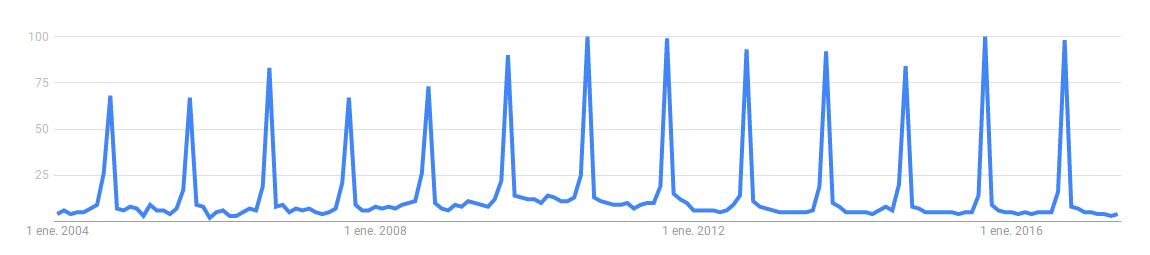
\includegraphics[width=15cm]{18_sept_google_trend.png}\\
	\caption{Frecuencia de consulta periódica: "18 de septiembre (2004-2016)". Fuente: Google Trends.}
	\label{fig:mesh1}
\end{figure}

\subsubsection{Consultas Ráfagas}
Este tipo de consultas se caracteriza principalmente por poseer una frecuencia constante en el tiempo, la cual se ve afectada por un evento en especifico ya sea de índole social, económico, cultural, etc. llamando así el interés de los usuarios en general. Provocando que la frecuencia respecto a un tema en especifico aumente bruscamente hasta alcanzar un pick, para luego ir reduciéndose a medida que pasa el tiempo, como consecuencia del desinterés que comienza a tener los usuarios respecto al tema mencionado. Un ejemplo de este tipo de consultas corresponde a la "muerte de Fidel Castro" tal como se muestra en la Figura \ref{google_trend_muerte_Fidel_Cast}.\\

\begin{figure}[!htb]
	\centering
	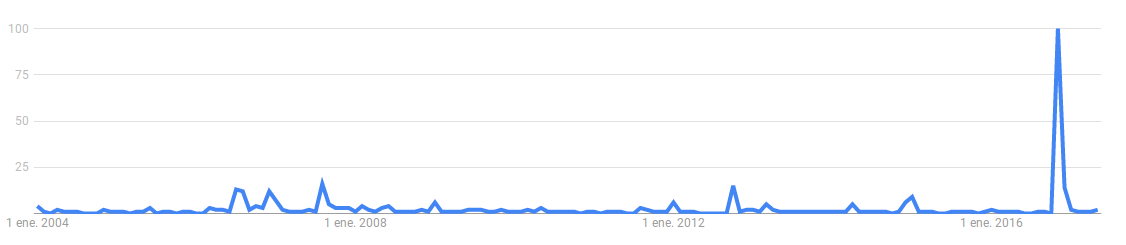
\includegraphics[width=15cm]{muerte_fidel_castro.png}\\
	\caption{Frecuencia de consulta ráfaga: "Muerte de Fidel Castro"(2004-2017). Fuente: Google Trends.}
	\label{google_trend_muerte_Fidel_Cast}
\end{figure}

Ademas, las consultas en ráfaga no solo afectan a una consulta en especifico, si no que también a todo conjunto de consultas que tengan algún tipo de relación con el evento especifico que llevo al alza en este topico. En la Figura \ref{google_trend_histo_Fidel_Cas} se puede observar como también la consulta "Historia de Fidel Castro" posee un patrón ráfaga de la misma forma que la consulta "muerte de Fidel Castro" y durante los mismos intervalos de tiempo.\\

\begin{figure}[!htb]
	\centering
	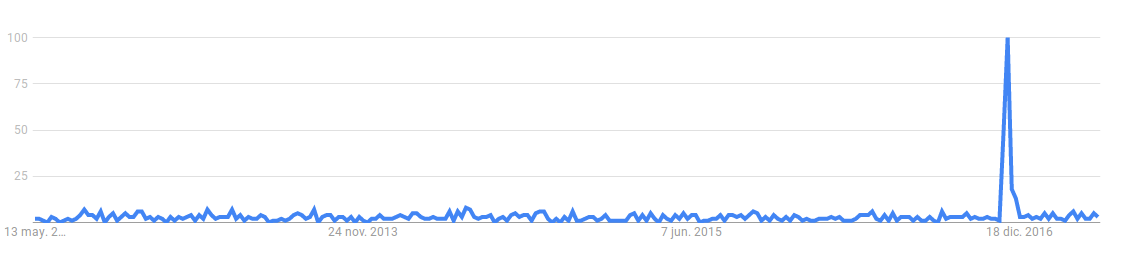
\includegraphics[width=15cm]{historia_Fidel_Castro.png}\\
	\caption{Frecuencia de consulta rafaga: "Historia de Fidel Castro"(2012-2017). Fuente: Google Trends.}
	\label{google_trend_histo_Fidel_Cas}
\end{figure}

Uno de los problemas mas serios que producen estas consultas debido al aumento en el volumen de consultas solicitadas, es la generación de desbalance en los nodos con respuestas pre-computadas en cache, como también una congestión al acceso de la información en los servidores.\\

\subsubsection{Consultas Permanentes}
Finalmente las consultas permanentes, son definidas como aquellas que poseen una continuidad en la frecuencia que son solicitadas en intervalos largo de tiempo, en simples palabras son consultas que el paso del tiempo no afecta abruptamente su frecuencia. En la Figura \ref{google_trend_google} se adjunta una consulta del tipo permanente la cual corresponde a "YouTube".\\

\begin{figure}[!htb]
	\centering
	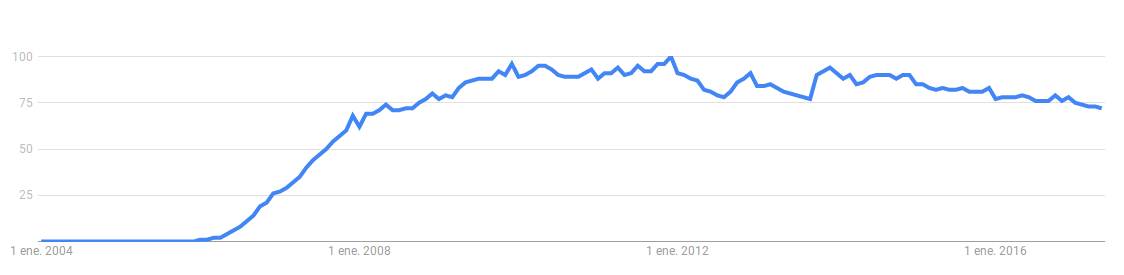
\includegraphics[width=15cm]{YouTube.png}\\
	\caption{Frecuencia de consulta permanente: "YouTube"(2004-2017). Fuente: Google Trends.}
	\label{google_trend_google}
\end{figure}

Bajo este contexto, muchos son los trabajos encontrados en la literatura \cite{zhang2013two}, \cite{markatos2001caching}, \cite{ozcan2012five}, \cite{kumar2008new}, los cuales tienen como conclusión que destinar un espacio estático en cache para guardar las consultas permanentes, lo que permite aumentar el rendimiento del cache, mejorando la tasa hit de este mismo. Cabe recordar que las consultas permanente se obtienen de registros históricos, los cuales son analizados para determinar cuales son consultas permanente y cuales no, tomando en cuenta su frecuencia. \\ 


%*******************************************************
\chapter{Estado del arte}
\section{NDNSIM}
\subsection{On Performance of Cache Policies in Named Data Networking}

En \cite{ran2013performance} se propone el diseño de una política de cache basada en la popularidad del contenido (CCP), la cual tiene en cuenta el factor de popularidad y una nueva estructura de datos denominada "Tabla de popularidad de contenido (CPT) sobre la base del Content Store (CS), Pending Interest Table (PIT) y la Forwarding Interest Base (FIB)

\section{Arquitectura de Caches}


%*******************************************************
%next line adds the Bibliography to the contents page
\addcontentsline{toc}{chapter}{Bibliography}
%uncomment next line to change bibliography name to references
%\renewcommand{\bibname}{References}
\bibliography{refs}        %use a bibtex bibliography file refs.bib
\bibliographystyle{plain}  %use the plain bibliography style

\end{document}

